\documentclass[12pt, letterpaper]{report}
\usepackage[margin=0.7in]{geometry}
\usepackage[utf8]{inputenc}
\usepackage{url}
\usepackage{hyperref}
\usepackage{graphicx}

\title{\Huge Guia de seguran\c{c}a para leigos}
\author{Gilgamesh}

\begin{document}
\maketitle
\pagebreak
\section*{Espionagem em massa - Um problema mundial}
\large Um dos maiores problemas na nossa sociedade moderna é a espionagem em masas. Governos roubam os teus dados, lhe espionagem e ainda dizem que é para o seu próprio bem.\\

	Depois dos vazamentos (leaks) feito por \textbf{Edward Snowden}, várias pessoas em todo o mundo passaram a se preocupar com a prórpia segurança e privacidade. Mas ainda assim, uma boa parcela da população não se preocupa com a própria privacidade e segurança, muitas vezes por não saber o que governos e empresas fazem com os dados coletados. Mas a população deveria sim se  preocupar com a privacidade, pois os mesmos métodos utilizado pelos governos para roubarem dados, também são utilizado por criminosos.\\

	A espionagem em massa acontece em todo e qualquer lugar do globo, não importa aonda você esteja, se tem algum meio de comunicação você está vulnerável à espionagem. Mesmo que você apenas utilize um telefone fixo, você está vulnerável à espionagem.\\

	As redes sociais atualmente é um dos maiores perigos para a segurança e privacidade dos usuários, visto que é possível determinar os seus gostos, seus amigos, sua família e diversas outras coisas. Sites como o Facebook, enquanto você o utiliza ele monitora o que você está acessando para poder lhe fazer propagandas direcionadas. O Google também faz isto. Embora seja a forma que estas empresas tem de ganhar dinheiro, é muito invasivo e na maioria das vezes não funciona. Mas para poder escapar desta vigilância, tem algumas coisas que podemos fazer.\\
	\begin{itemize}
		\item Utilize o redes sociais apenas quando necessário.
		\item Sempre que for utilizar alguma rede social, utilize-a com alguma \href{https://criptowiki.miraheze.org/wiki/VPN_(Virtual_Private_Network)}{VPN}.
		\item Se não for necessário ter uma rede social, não tenha.
	\end{itemize}
\pagebreak
%Segurança na internet.
\section*{Segurança na internet}
	A internet é um lugar vasto, mas com vários perigos. Estamos na era da informação, na qual tudo (ou quase tudo) é feito pela internet, e justamente por isso que ela se tornou extremamente perigosa para usuários leigos. Os perigos que corremos não é apenas por criminosos, mas também pelo estado.\\

	Um dos maiores perigos que temos são os ataques de \href{https://criptowiki.miraheze.org/wiki/Phishing}{phishing}, que consiste basicamente em uma clonagem de sites feitos na rede interna ou não e que tem como objetivo roubar dados do usuário, como login e senha de bancos e de redes sociais.\\

	Mas os ataques de phishing tem alguns erros na qual é possível usuários identificarem se estão em um site falso. Um método de verificar se o site é falso ou não, é através da URL (endereço) do site, que \textbf{pode} estar errada e assim o usuário poderá saber se está sendo vítima de um ataque phishing. Então a dica é ficar atento à URL do site.\\

	E uma outra forma além de verificar o endereço URL é verificar o \textbf{certificado SSL}, que é basicamente um protocolo de rede que garante que o site é verídico e que é utilizado junto ao protocolo \textbf{HTTPS}. Em casos de phishing na rede interna, quando o indivíduo invade a rede WiFi, é possível verificar o certificado SSL. Quando você acessar um site de banco ou algum site importante, fique atento ao cadeado verde que aparece perto à barra de endereço.

	\begin{center}
		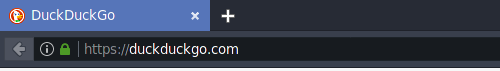
\includegraphics[scale=1]{Duck.png}\\
		\footnotesize O cadeado verde representa o certíficado SSL
	\end{center}

	O certíficado SSL nem sempre está nos sites, principalmente em sites pequenos, é comum eles não terem um certíficado SSL. Mas caso aconteça de algum site importante, como o site do Facebook ou o site do teu banco não tenha certíficado SSL, é recomendavel não fazer login.\\

\pagebreak

	Os \href{https://criptowiki.miraheze.org/wiki/Spam}{spam} foram um método muito utilizado como forma de espalhar malwares e também para poder fazer phishing em usuários.\\

	Os spams são basicamente mensagens enviada para e-mails aleatórios com algum link para o usuário acessar ou algum arquivo para baixar. Eles foram e ainda é bem comum, embora não seja um método muito eficaz atualmente, mas caso receba alguma mensagem por e-mail com um título sensacionalista, é recomendavel não abri-lo. Então a dica é que antes de abrir uma mensagem de e-mail, pense 2 vezes ao abri-lo e se abrir, pense bem antes de clicar em algo.\\

	Os arquivos e programas que são baixados na internet, muitas vezes podem vir com algum software malicioso junto ao arquivo ou programa baixado, desta forma, dando ao invasor total controle da máquina. Se for baixar algum arquivo ou software, certifique que ele está sendo baixado do site oficial ou até mesmo pela loja de software do sistema operacional.\\

\pagebreak

\section*{DNS}
	O \href{https://criptowiki.miraheze.org/wiki/DNS_(Domain_Name_System)}{DNS} (\textbf{Domain name System}) é o responsável por levar o usuário até o site desejado.\\
	Suponha-se que o usuário deseja ir até o site \textbf{google.com}, para que ele possa ir até o site, é necessário ir até o \href{https://pt.wikipedia.org/wiki/IP}{IP} correspondente do site. O DNS é o responsável por levar o usuário até o IP correspondente ao site.
	O servidor DNS interfere e muito na velocidade da conexão e também é possível que o servidor DNS seja invadido por alguém mal intencionado e utilizar o servidor DNS para que possa fazer um ataque phishing e assim fazer todos os usuários que utilizam aquele servidor acreditar que o site que está sendo acessado é o verdadeiro, quando na verdade é um site falso.\\

	Neste ano houve um caso na qual um servidor DNS foi invadido no terceiro dia deste ano (2017) e o site do Google aparecia uma imagem diferente:

\begin{center}
	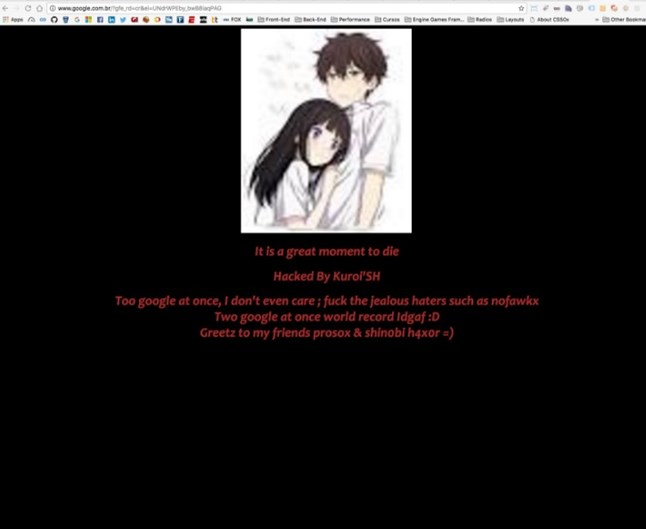
\includegraphics[scale=0.7]{dns.jpg}\\
\end{center}

	Geralmente, usuários não configuram o servidor DNS que será utilizado pelo sistema e por padrão, o sistema utiliza o servidor DNS oferecido pelo próprio provedor de internet, o que pode não ser uma boa ideia visto que ISP (Internet Service Provider) pode ser infectado fácilmente e que ele não é especializado nisto.\\

	Existem diversos servidores DNS seguros e que são recomendados e utilizados por técnicos em segurança.\\

	Servidores DNS recomendados:

	\begin{itemize}
		\item OpenDNS
		\item Google DNS
		\item DynDNS
	\end{itemize}

	Para poder configurar o servidor DNS que será utilizado é bastante simples e por isto não irei demonstrar aqui, basta uma rápida pesquisa em algum site de busca para que você possa encontrar tutoriais.\\

\pagebreak

\section*{Segurança nos sistemas operacionais}
	Os sistemas operacionais (\textbf{OS}) é a parte mais importante de um computador. É onde tudo ocorre, é onde o usuário usa a internet, edita documentos, guarda documentos e várias outras atividades e é exatamente por isto que deve-se mante-lo seguro e livre de ameaças.\\

	O sistema operacional para computadores mais utilizados atualmente é o Windows. Embora o Windows seja considerado por muitos como o melhor sistema operacional, na realidade não é bem assim. O Windows é um sistema operacional totalmente fechado, que quer dizer que nenhuma linha de código do sistema está exposto para que o usuário possa ver. Por este motivo, caso a Microsfot  deseje, ela pode colocar algum \href{https://criptowiki.miraheze.org/wiki/Backdoors}{backdoor} no OS e assim, não apenas a Microsoft mas também qualquer pessoa mal intencionada poderia fazer uso deste backdoor para poder controlar a máquina e roubar dados do usuário.\\

	Além do Windows ser um sistema fechado, ele também tem diversas vulnerabilidades e que não são exploradas apenas por hackers mas também por governos, como é o caso dos recentes vazamentos de ferramentas que eram utilizadas pela NSA para poder explorar vulnerablidades no protocolo SMB do Windows. Estas ferramentas que eram utilizadas pela NSA para explorar falhas no protocolo SMB, foram vazadas pelo grupo \textbf{Shadown Brokers}. Estas ferramentas foram utilizadas para criar o WannaCry que é um \href{https://criptowiki.miraheze.org/wiki/Ransomwares}{ransomware}. Este ransomware infectou milhares de máquinas em todo o mundo e gerou uma grande repercução em todo o globo pelo seu tempo de propagação que durou horas e que já tinha infectado vários países.\\

\begin{center}
	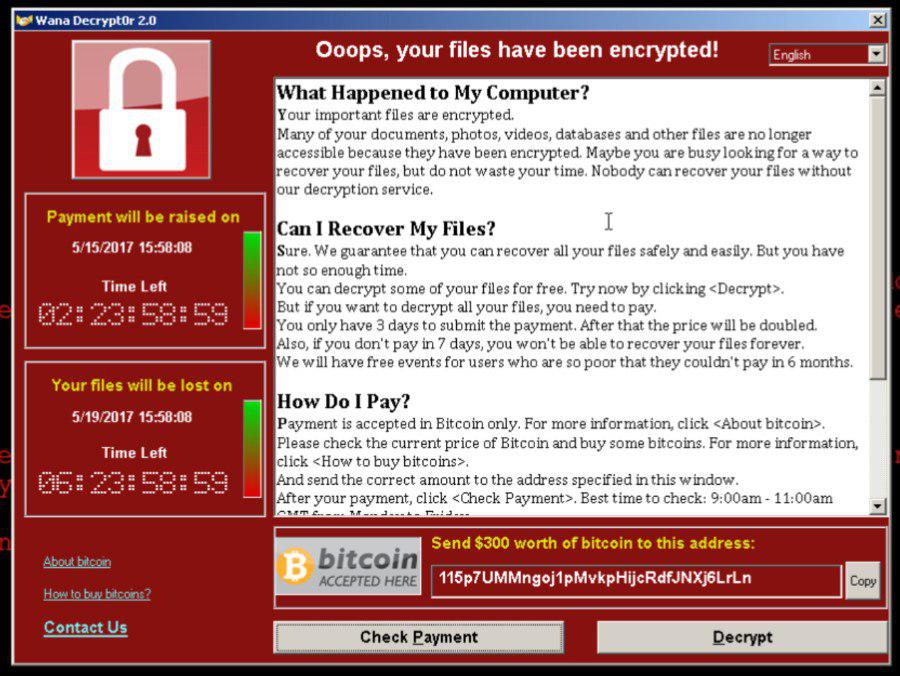
\includegraphics[scale=0.8]{wannacry.jpg}\\
	\footnotesize WannaCry
\end{center}

	Além do Windows ser um OS com várias falhas, também é um sistema que "espiona" os usuários, mandando diversas informações para os servidores da Microsoft e assim corrompendo a privacidade dos usuários. Um outro ponto negativo no Windows é o tempo de correção de falhas que podem durar semanas ou até meses ({\textit alguns casos demoraram até 6 meses}), o que é extremamente ruim para os usuários que ficam vulneraveis durante meses e as ferramentas para explorar estas falhas estão na internet para que qualquer um possa utiliza-las.\\

	Em distribuições Linux, na qual o código fonte dos programas e do sistema operacional é aberto para que qualquer um possa olhar, as correções de falhas podem durar alguns dias ou ({/textbf raramente}) alguns dias. E também, distribuições Linux tem poucas falhas. Mais para frente, irei falar um pouco sobre o Linux.\\

	Em geral, existem falhas, mas ainda assim é bom o usuário ficar atento e manter o sistema seguro. As dicas dada por profissionais de segurança são:

	\begin{itemize}
		\item Manter o sistema atualizado.
		\item Não baixar softwares de sites não confiaveis
		\item Não baixar arquivos que não se sabe de quem ou o que é.
		\item Sempre baixar softwares dos sites ou repositórios oficiais.
		\item Usar softwares renomados e que de preferência seja OpenSource.
		\item Manter backups constantes de arquivos importantes.
	\end{itemize}

	Estas dicas são básicas, porém é recomendado segui-las para que os usuários não sejam tão fácilmente infectados por malwares.




\end{document}
